\input{Math Club W10/Packages}
\input{Math Club W10/Definitions}

\fancypagestyle{firstpageheader}{
    \fancyhf{}
% Header
    \fancyhead[L]{\MathClubW{10}}
    \fancyhead[R]{11/25/2024}
% Footer
    \fancyfoot[C]{\thepage}
    \renewcommand{\headrulewidth}{0.4pt} 
}

\parindent 0pt
\marginparsep 3pt

\clubpenalty=500 % Control break penalty for single lines at top
\widowpenalty=500 % Control break penalty for single lines at bottom
\displaywidowpenalty=500
\interlinepenalty=0 % Encourage breaks between lines

\begin{document}

\sloppy
\thispagestyle{firstpageheader}

\section*{AMATYC problems}

\begin{problem}[C][1][AMATYC Spring 2019/10]
     % Discrete ^ Student Math League
     Morse code involves transmitting dots “•” and dashes “\textsf{---}”. An agent attempted to send a five-character code five different times, but only one of the five transmissions was correct. However, it was known that each erroneous transmission had a different number of errors than the others, and no transmission had five errors. The first transmission was • \textsf{---} \textsf{---} • \textsf{---}, which was not correct. The other four transmissions are listed below. Which one is correct? 
\end{problem}
\multOpt[5]{• \textsf{---} \textsf{---} \textsf{---} •}
[\textsf{---} \textsf{---} • • \textsf{---}][• \textsf{---} • \textsf{---} •][• • • • •][Impossible to determine]

\begin{solution}[A]
    Between the four erroneous transmissions, there could be 1, 2, 3, 4, or 5 errors. But since none of the five transmissions are exact opposites of another, there is exactly one transmission with 1, 2, 3, and 4 errors, and a correct transmission. 
    
    A has 2 differences with G (given), 4 differences with B, 1 difference with C, and 3 differences with D.

    B can't be correct, since it has 3 differences with both C and D.

    C can't be correct, since it has 3 differences with both G and B.

    D can't be correct, since it has 3 differences with both G and A.

    So \fbox{A} is the correct transmission.
\end{solution}

\begin{problem}[C][3][AMATYC April 2002/6]
    % Divisibility ^ Simon's Favorite Factoring Trick ^ Student Math League
    In how many different ways can $\frac{2}{15}$ be represented as $\frac{1}{a}+\frac{1}{b}$ where $a$ and $b$ are positive integers with $a>b$
\end{problem}
\multOpt[5]{1}[2][3][4][More than 4]

\begin{solution}[D]
    We start by rearranging the original equation:
    \begin{align*}
        &\frac{1}{a}+\frac{1}{b}=\frac{2}{15}\\
        \iff &15(a+b)=2ab\\
        \iff &2ab-15a-15b=0\\
        \iff &4ab-30a-30b+225=225\\
        \iff &(2a-15)(2b-15)=225
    \end{align*}
    Then $(2a-15)$ and $(2b-15)$ are factors of $225=3^2 \cdot5^2$ , this gives:\\
    $(2a-15,2b-15) = (225,1),(75,3),(45,5),(25,9)$ (note that we excluded $(15,15)$ since $a>b$)\\
    This further implies $(a,b) = (30,10),(45,9),(20,12),(120,8)$
\end{solution}

\begin{problem}[A][3][AMATYC Spring 2007/8]
    % Functionals ^ Algebra ^ Student Math League
    A function $f$ is symmetric to the origin and periodic with period 8. If $f(2) = 3$, what is the value of $f(4) + f(6)$?
\end{problem}
\multOpt[5]{$-6$}[$-3$][$0$][$3$][$6$]

\begin{solution}[B]
    Symmetry about the origin means (i) $f(a)=-f(-a)$ and 8-periodicity means (ii) $f(a)=f(a\pm8k)$. 

    Finding $f(6)$ is relatively simple, since using (i) and then (ii) we get $f(6) = -f(-6) = -f(2) = -3$.

    To find $f(4)$, observe that (i) gives $f(-4) = -f(4)$ and (ii) gives $f(-4) = f(4)$. So $-f(4)=f(4)$ and thus we could only have $f(4)=0$.

    Therefore $f(4) + f(6) = 0 + (-3) = \boxed{-3}$.
\end{solution}

\begin{problem}[C][5][AMATYC Fall 2001/8]
    % Algebra ^ Student Math League
    The letters of \texttt{AMATYC} are replaced by distinct digits from 0 to 9 (so that different letters represent different digits). If the 3-digit integer \texttt{AMA} is a perfect cube, and the 3-digit integer \texttt{TYC} is a perfect square divisible by 12, what is \( A + M + A + T + Y + C \)?
\end{problem}
\multOpt[5]{19}[21][25][28][37]

\begin{solution}[D]
    The key detail to find possible solutions is realizing that there aren't many possibilities for both \texttt{AMA} and \texttt{TYC}, for example the smallest three-digit cube is $5^3=125$ and the largest is $10^9=729$, thus $\texttt{AMA} \in \{ 5^3,6^3,7^3,8^3,9^3\}= \{ 125,216,343,512,729\}$, since the only case that has the first and last digit equal is 343, this must be equal to \texttt{AMA}.
    
    In a similar way, the smallest three-digit square is $10^2=100$ and the largest is $31^2=961$, but since \texttt{AMA} is divisible by 12 we can narrow down our options to $\texttt{TYC} \in \{12^2,18^2,24^2,30^2 \} = \{144,324,576,900 \}$, then \texttt{TYC}=576 since $M=4$ and $900$ has repeating digits.
    
    We conclude $ A + M + A + T + Y + C =3+4+3+5+7+6= \boxed{28} $
\end{solution}

\begin{problem}[R][3][AMATYC Fall 2001/17]
    % Derivatives ^ Inequalities ^ Student Math League
    If \( n \) positive integers have a sum of 10, what is the maximum possible value of their product?
\end{problem}
\multOpt[5]{30}[32][36][40][45]

\begin{solution}[C]
    The AM-GM (arithmetic/geometric mean) inequality tells us that
    \[
        \sqrt[n]{x_1 \cdot x_2 \cdot \dots \cdot x_n} \leq \frac{x_1 + x_2 + \dots + x_n}{n} \quad \iff \quad x_1 \cdot x_2 \cdot \dots \cdot x_n \leq \left(\frac{x_1 + x_2 + \dots + x_n}{n}\right)^{\!\!n}
    \]
    Replacing the sum with 10 and plugging in values of $n$, we find that the product is maximized for $n=4$:
    \[
    \max\!\left[ \left(\frac{10} {n}\right)^{\!\!n}\, \right] =\displaystyle \left(\frac{10} {4}\right)^{\!\!4} \approx 39
    \]
    The nearest solution below $39$ is $36$. To verify $36$ as a possible product, observe that $10/4=2.5$ and pick $3$ or $4$ numbers close to $2.5$ to see if they add to 10 and multiply to 36. Two such sets are $\{2,2,3,3\}$ and $\{3,3,4\}$. So our solution is \fbox{36}.
\end{solution}

\newpageSol

\begin{problem}[N][4][AMATYC Fall 2007/18]
    % Divisibility ^ Simon's Favorite Factoring Trick ^ Student Math League
    Let \( r, s, \) and \( t \) be nonnegative integers. Find the number of triples \( (r, s, t) \) which satisfy:\vspace{-2mm}
    \begin{align*}
        rs + t &= 14 \\
        r + st &= 13
    \end{align*}
\end{problem}\vspace{-3mm}
\multOpt[5]{2}[3][4][5][6]

\begin{solution}[A]
    Subtract the equations to get $rs-r+t-st=(r-t)(s-1)=1$, thus $(r,s,t)=(5,2,4) , (13,0,14)$. $\Box$
\end{solution}

\begin{problem}[P][7][AMATYC Fall 2014/10]
    % Algebra ^ Probability ^ Student Math League
    You win a certain game by either pushing a button once and getting a green light, or pushing the button twice and getting either 2 green lights or exactly one red light. The probability $p > 0$ of a green light on a single push is constant and three times the probability of a red light. Find the value of $p$ for which the probability of winning is the same for either the one-push or two-push option.
\end{problem}
\multOpt[5]{3/8}[3/7][2/5][1/2][3/5]

\begin{solution}[B]
    We know that on any single push, the probability of getting a green light is $P(G)=p$ and the probability of getting a red light is $P(R)=\frac{1}{3}p$. Thus, with $W_n$ denoting a win from $n$ pushes, we have
    \begin{alignat*}{3}
        P(W_1) &= P(G) &&= p\\
        P(W_2) &= [P(G) \cdot P(G)] + 2[P(R) \cdot P(\neg R)] = p^2 + 2\left(\tfrac{1}{3}p\right)\left(1-\tfrac{1}{3}p\right) &&= \tfrac{7}{9}p^2 + \tfrac{2}{3}p
    \end{alignat*}
    Setting $P(W_1)=P(W_2)$ we get
    \[
        \tfrac{7}{9}p^2 + \tfrac{2}{3}p = p \quad \Rightarrow \quad 7p^2 - 3p = 0 \quad \Rightarrow \quad p = \boxed{\tfrac{3}{7}}
    \]
\end{solution}

\newpage
\section*{I want to be fried in an oven}

\begin{problem}[R][3][Putnam 2016 /A1]
    % Pigeonhole Principle ^ Divisibility ^ Derivatives ^ Putnam
    Find the smallest positive integer \( j \) such that for every polynomial \( p(x) \) with integer coefficients and for every \( k \), the integer
\[
p^{(j)}(k) = \frac{d^j}{dx^j}p(x) \bigg|_{x=k}
\]
(the \( j \)-th derivative of \( p(x) \) at \( k \)) is divisible by 2016.
\end{problem}

\begin{solution}[8]
    We need 2016 to divide the coefficient of every term of $p^{(j)}(x)$. Without loss of generality, we'll assume every coefficient in the original $p(x)$ is $1$. Considering the $n$-th term of $p(x)$, observe that
    \begin{align*}
        \frac{d^j}{dx^j}x^n = 0 \quad \text{for}\ n < j \qquad \qquad \frac{d^j}{dx^j}x^n = \frac{n!}{(n-j)!}x^{n-j} \quad \text{for}\ n \geq j
    \end{align*}
    So terms of degree $n<j$ are all $0$, which 2016 divides. The remaining terms have coefficients of form
    \begin{align*}
        c_n = \frac{n!}{(n-j)!} = (n)(n-1)(n-2)\dots(n-(j-1)) = \prod_{i=0}^{j-1}(n-i)
    \end{align*}
    So to get $2016 \mid c_n$, we must find the smallest $j$ such that the 2016 divides any product of $j$ consecutive integers, using the fact that $2016 = 2^5 \cdot 3^2 \cdot 7$. This immediately tells us that we must have $j \geq 7$ for $7 \mid c_n$, because 7 divides only one in every seven consecutive integers. We also know 3 divides one in every three consecutive integers and thus two in every six, meaning $3^2 \mid c_n$ for all $j \geq 7$ as well. However, $j = 7$ is not sufficient for $2^5 \mid c_n$. Out of seven factors, three will be a multiple of 2 and one of these will be a multiple of 4, but this guarantees us divisibility by $2^4$ only. Thus, the smallest possible $j$ is $j =\boxed{8}$.
\end{solution}

\begin{problem}[R][7][Putnam 2018 /B2]
    % Complex Numbers ^ Algebra ^ Putnam
    Let $n$ be a positive integer and let $f_n(z)=n+(n-1)z+(n-2)z^2+\ldots+z^{n-1}$. Prove that $f_n$ has no roots in the closed unit disk. $\{z \in \mathbb{C}:|z| \leq 1 \}$
\end{problem}

\begin{solution}
    Note that:
    \begin{align*}
        f_n(z)=\sum_{i=0}^{n-1}(1+z+\ldots+z^i) = \sum_{i=0}^{n-1}\left(\frac{z^{i+1}-1}{z-1}\right)\\
        \iff (z-1)f_n(z)=z+z^2+\ldots+z^n-n
    \end{align*}
    If $f_n(z)=0$ with $|z|\leq 1$, recall that $\forall a,b :|a|+|b|\leq|a+b|$ and that $|z|\leq 1 \Rightarrow|z^k| \leq 1$ to see that $|z+z^2+\ldots+z^n| \leq n$. So if we want $f_n(z)=0$ then it corresponds to the equality case when $|z|=|z^2|=\ldots=|z^n|$, this happens when $z=1$, but $f_n(1) \neq 0$ , so we can't have a root $z$ with $|z| \leq 1$ $\Box$
\end{solution}

\begin{problem}[C][7][Putnam 2020 /A2]
    % Algebra ^ Double Counting ^ Induction ^ Putnam
    Evaluate
    $$\sum_{j=0}^k 2^{k-j} \binom{k+j}{j}$$
\end{problem}

\begin{solution}[$4^k$]
    Consider a very important meeting of $2k$ persons that wanted to decide whether dogs or cats are the best. Each person has a seat at a circular table and then decides between cats and dogs.
    
    We will count all the possible ways in which this meeting can happen in two different ways. First, see that each person can choose any option independently, giving $2^{2k}=4^k$ possible ways to conclude the meeting.

    On the other hand, we say that a transition happens if a person does not agree with the person on his left, say we have $j$ transitions and fix $0\leq j \leq k$. Because we will introduce all the $j$ transitions only between the last $k$ people, this is equivalent to selecting $j$ slots out of $k+j$ possibilities, giving $\binom{k+j}{j}$ ways to do this. 
    
    Also, the remaining $k-j$ persons can choose either dogs or cats, giving $2^{k-j}$ possibilities. Thus we have $2^{k-j}\binom{k+j}{j}$ choices for $j$ transitions, since we counted all possibilities in two different ways, these must be equal: 
    $$\sum_{j=0}^k 2^{k-j} \binom{k+j}{j}=4^k $$
    For example, if $k=3$ and $j=2$ , there are 6 people and one person ($k-j=1$) was not selected for the transition, say WLOG that this person selected dogs (D), then in the remaining $k+j=5$ persons, there are 2 transitioned people (colored in red) and 3 stationary (not transitioned) people (colored in blue). The $\binom{3+2}{2}=10$ possibilities for table arrangements are:
    
    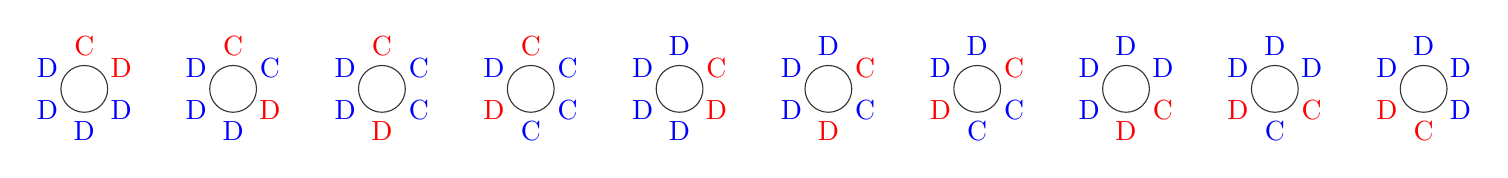
\begin{tikzpicture}[scale=0.54]
        % 1. CDDDD
        \draw[black!80] (0,0) circle (0.55);
        \node[red] at (90:1) {C};
        \node[red] at (30:1) {D};
        \node[blue] at (-30:1) {D};
        \node[blue] at (-90:1) {D};
        \node[blue] at (-150:1) {D};
        \node[blue] at (150:1) {D};
        
        % 2. CCDDD
        \begin{scope}[xshift=3.5cm]
        \draw[black!80] (0,0) circle (0.55);
        \node[red] at (90:1) {C};
        \node[blue] at (30:1) {C};
        \node[red] at (-30:1) {D};
        \node[blue] at (-90:1) {D};
        \node[blue] at (-150:1) {D};
        \node[blue] at (150:1) {D};
        \end{scope}
        
        % 3. CCCDD
        \begin{scope}[xshift=7cm]
        \draw[black!80] (0,0) circle (0.55);
        \node[red] at (90:1) {C};
        \node[blue] at (30:1) {C};
        \node[blue] at (-30:1) {C};
        \node[red] at (-90:1) {D};
        \node[blue] at (-150:1) {D};
        \node[blue] at (150:1) {D};
        \end{scope}
        
        % 4. CCCCD
        \begin{scope}[xshift=10.5cm]
        \draw[black!80] (0,0) circle (0.55);
        \node[red] at (90:1) {C};
        \node[blue] at (30:1) {C};
        \node[blue] at (-30:1) {C};
        \node[blue] at (-90:1) {C};
        \node[red] at (-150:1) {D};
        \node[blue] at (150:1) {D};
        \end{scope}
        
        % 5. DCDD
        \begin{scope}[xshift=14cm]
        \draw[black!80] (0,0) circle (0.55);
        \node[blue] at (90:1) {D};
        \node[red] at (30:1) {C};
        \node[red] at (-30:1) {D};
        \node[blue] at (-90:1) {D};
        \node[blue] at (-150:1) {D};
        \node[blue] at (150:1) {D};
        \end{scope}
        
        % 6. DCCDD
        \begin{scope}[xshift=17.5cm]
        \draw[black!80] (0,0) circle (0.55);
        \node[blue] at (90:1) {D};
        \node[red] at (30:1) {C};
        \node[blue] at (-30:1) {C};
        \node[red] at (-90:1) {D};
        \node[blue] at (-150:1) {D};
        \node[blue] at (150:1) {D};
        \end{scope}
        
        % 7. DCCCD
        \begin{scope}[xshift=21cm]
        \draw[black!80] (0,0) circle (0.55);
        \node[blue] at (90:1) {D};
        \node[red] at (30:1) {C};
        \node[blue] at (-30:1) {C};
        \node[blue] at (-90:1) {C};
        \node[red] at (-150:1) {D};
        \node[blue] at (150:1) {D};
        \end{scope}
        
        % 8. DDCDD
        \begin{scope}[xshift=24.5cm]
        \draw[black!80] (0,0) circle (0.55);
        \node[blue] at (90:1) {D};
        \node[blue] at (30:1) {D};
        \node[red] at (-30:1) {C};
        \node[red] at (-90:1) {D};
        \node[blue] at (-150:1) {D};
        \node[blue] at (150:1) {D};
        \end{scope}
        
        % 9. DDCCD
        \begin{scope}[xshift=28cm]
        \draw[black!80] (0,0) circle (0.55);
        \node[blue] at (90:1) {D};
        \node[blue] at (30:1) {D};
        \node[red] at (-30:1) {C};
        \node[blue] at (-90:1) {C};
        \node[red] at (-150:1) {D};
        \node[blue] at (150:1) {D};
        \end{scope}
        
        % 10. DDDCD
        \begin{scope}[xshift=31.5cm]
        \draw[black!80] (0,0) circle (0.55);
        \node[blue] at (90:1) {D};
        \node[blue] at (30:1) {D};
        \node[blue] at (-30:1) {D};
        \node[red] at (-90:1) {C};
        \node[red] at (-150:1) {D};
        \node[blue] at (150:1) {D};
        \end{scope}
    \end{tikzpicture}
\end{solution}

\begin{solution}[Alternative way using induction]
    It is easy to check that the given expression is $4^k$ when $k=0$, this will be the base case of our induction.\\
    Let's assume that if
    $$\sum_{j=0}^k 2^{k-j} \binom{k+j}{j}=4^k$$
    then it implies
    $$\sum_{j=0}^{k+1} 2^{k+1-j} \binom{k+1+j}{j}=4^{k+1}$$
    We will two identities (they aren't hard to prove):
    \begin{align}
        \binom{n}{r}+\binom{n}{r-1}&=\binom{n+1}{r} \text{\hspace{7pt} (Pascal Identity)}\\
        \binom{n+1}{r+1} &= \frac{n+1}{r+1} \binom{n}{r}
    \end{align}
    They are useful because they relate $n+1$ to $n$, this is essential while using induction.
    \begin{align*}
        \mathop{\textcolor{blue}{\sum}}_{j=0}^{k+1} 2^{k+1-j} \binom{k+1+j}{j}
        & =\sum_{j=0}^{k} 2^{k+1-j} \binom{k+1+j}{j} + \binom{2k+2}{k+1}\\
        &= \sum_{j=0}^{k} 2^{k+1-j} \binom{k+j}{j} + \sum_{j=1}^{k} 2^{k+1-j} \binom{k+j}{j-1}+\binom{2k+2}{k+1} \text{\hspace{10pt} by (1)}\\
        &= 2\cdot4^k + \sum_{i=0}^{k-1} 2^{k-i} \binom{k+1+i}{i}+\binom{2k+2}{k+1}\\
        &= 2\cdot4^k + 2^{-1}\sum_{i=0}^{k-1} 2^{k+1-i} \binom{k+1+i}{i}+\binom{2k+1}{k}+2^{-1}\binom{2k+2}{k+1} \text{\hspace{10pt} by (2)}\\
        &= 2\cdot4^k + 2^{-1}\mathop{\textcolor{blue}{\sum}}_{i=0}^{k+1} 2^{k+1-i} \binom{k+1+i}{i}\\
    \end{align*}
    Then
    \begin{align*}
        \frac{1}{2} \mathop{\textcolor{blue}{\sum}}_{j=0}^{k+1} 2^{k+1-j} \binom{k+1+j}{j} = 2 \cdot 4^k \\
        \iff \mathop{\textcolor{blue}{\sum}}_{j=0}^{k+1} 2^{k+1-j} \binom{k+1+j}{j} = 4^{k+1}\\
        \Box
    \end{align*}
\end{solution}

\begin{problem}[Q][5][44th Spanish Mathematical Olympiad P2]
   % Inequalities 
    Show that for any real numbers $a,b$ such that $0<a,b<1$, the following inequality holds:
    $$\sqrt{ab^2+a^2b} + \sqrt{(1-a)(1-b)^2+(1-a)^2(1-b)} < \sqrt2$$
\end{problem}

\begin{solution}
    For the sake of symmetry, I will define $c=1-a$ and $d=1-b$, and call $S=\sqrt{ab^2+a^2b}+\sqrt{cd^2+c^2d}$; thus we want to prove $S<\sqrt2$. By the Cauchy-Schwarz inequality, we have that:
    \begin{align*}
        (ab+cd)(a+b+c+d) \geq S^2\\
        \iff 2(ab+cd) \geq S^2
    \end{align*}
    So we have to show that $1>ab+cd$ to conclude, this is true because:
    \begin{align*}
        &ab+cd<1 \\
         \iff &ab+(1-a-b+ab)<1 \\
        \iff &2ab<a+b \iff 2 < \frac{1}{a} + \frac{1}{b}
    \end{align*}
    Which is clearly true because $0<a,b<1 \hspace{7pt} \Box$
\end{solution}

\begin{problem}[G][6][Putnam 2016 /B3]
    % Discrete ^ Geometry ^ Pigeonhole Principle
    Suppose that $S$ is a finite set of points in the plane such that the area of triangle $\triangle ABC$ is at most 1 whenever $A, B$, and $C$ are in $S$. Show that there exists a triangle of area 4 that (together with its interior) covers the set $S$.
\end{problem}

\begin{solution}
    Let $A,B,C$ be three points in S such that the area of $\triangle ABC$ is maximized, then we will see that the space on the plane in which any point $P \in S$ can exist is precisely a triangle with area at most $4$.\\
    Let $\ell_1,\ell_2,\ell_3$ be the lines parallel to $AB,BC $ and $AC$ respectively.
    Since the area of $\triangle PAB$ can't be greater than $\triangle ABC$, $P$ must be in the half-plane bounded by $\ell_1$ that contains $A$ and $B$. In a similar way, since the area of $\triangle PBC$ can't be greater than the area of $\triangle ABC$, then $P$ is in the half-plane bounded by $\ell_2$ that contains $B$ and $C$; the same argument goes for $\ell_3$.\\
    So we must have $P$ inside the intersections of $\ell_1,\ell_2$ and $\ell_3$, this is a triangle with area at most 4. $\Box$

    \begin{center}
    \begin{tikzpicture}
    
        \def\radius{6} \def\X{0.35} \def\labelSpacing{1.1}
        \def\X{110} \def\Y{210} \def\Z{350}
    
        \tkzDefPoints{0/0/O, \radius/0/R} % defines the first two points
        \tkzDefPointBy[rotation=center O angle \X](R)\tkzGetPoint{X}
        \tkzDefPointBy[rotation=center O angle \Y](R)\tkzGetPoint{Y}
        \tkzDefPointBy[rotation=center O angle \Z](R)\tkzGetPoint{Z}
    
        \tkzDefMidPoint(Y,Z)\tkzGetPoint{A}
        \tkzDefMidPoint(X,Z)\tkzGetPoint{B}
        \tkzDefMidPoint(X,Y)\tkzGetPoint{C}
        
        \tkzDrawSegments[dash pattern=on 5pt off 5pt](X,Y Y,Z Z,X)
        \tkzDrawSegments(A,B B,C C,A)
        
        \tkzLabelPoints[below](A){A}
        \tkzLabelPoints[left](C){C}
        \tkzLabelPoints[right](B){B}
        \tkzLabelSegment[left,pos=0.2](X,Y){$\ell_1$}
        \tkzLabelSegment[below,pos=0.2](Y,Z){$\ell_2$}
        \tkzLabelSegment[above,pos=0.8](X,Z){$\ell_3$}
    \end{tikzpicture}
    \end{center}
    Note: The reasoning for defining $\ell_1,\ell_2$ and $\ell_3$ comes from the fact that in any triangle $ABC$, if we move $A$ through the line parallel to $BC$ that contains $A$, then the area of $\triangle ABC$ will remain constant (base times height).\\
    The problem asks for a triangle of area 4, but if it has area $k<4$ we can just get a bigger triangle scaling the original one by $4/k$, which obviously meets all the conditions as well.
\end{solution}

\end{document}